\section{Reading zero modes by orthogonal branches}
\label{sec:flags}

We now turn the pinning maps into coordinates on every zero space.  At
each step we either record a hole or remove an electron.  The coordinates
are orthogonal, although the holes themselves have not been assigned
positions.  The purpose of the construction is quantitative: a local
observable near the north pole can change substantially only when the
coordinates record a hole sufficiently far along the descent toward that
pole.  We prove this assertion as an operator inequality, and then use
rotation averaging to obtain a uniform comparison in the one-hole spaces.

Throughout this section, all lower bounds on the flux are absorbed into
one fixed integer $q_{\mathrm{stop}}\geq 4$.  We stop every descent when
$q\leq q_{\mathrm{stop}}$.  Constants may depend on this stopping value,
on the uniform constants of the local calculus, and on a fixed decay
exponent.  They never depend on $q$ or on the particle number.

\subsection{The algebraic decomposition}

Let $P_q$ be the orthogonal projection onto the Fock zero space
$Z_q=\bigoplus_n Z_{n,q}$.  Write $n_q=c_q^*c_q$ for occupation of the
south-pole orbital.  In a nonzero sector $Z_{n,q}$ set
\begin{equation}
 h=q+3-3n.
 \label{eq:flags-hole-count}
\end{equation}
For $n\geq 1$, divisibility by the cube of every pair determinant gives
\begin{equation}
 Z_{n,q}=\left\{
  \prod_{i<j}(z_{i0}z_{j1}-z_{j0}z_{i1})^3 S:
  S\text{ is symmetric and homogeneous of degree }h
       \text{ in each spinor}\right\}.
 \label{eq:flags-polynomial-space}
\end{equation}
Thus $h\geq0$.  We retain Equation~\eqref{eq:flags-hole-count} also in
the vacuum sector, where $h=q+3$.

Denote by $Z_{n,q}^{(d)}$ the subspace in which each electron has $d$
zeros at the south pole.  The endpoint transport from
Section~\ref{sec:pinning}, followed by the inclusion with its last $d$
orbitals vacant, will be denoted by
\[
 \mathcal U_{q,d}:Z_{n,q-d}\longrightarrow Z_{n,q}^{(d)},
 \qquad d\in\{1,3\}.
\]
It is an isometry, preserves particle number and the sum of the orbital
indices, and is defined with the same choices on all number sectors.

\begin{lemma}[Two orthogonal branches]
\label{lem:flags-branch-algebra}
For $q>q_{\mathrm{stop}}$, define
\[
 \mathcal F_{n,q}=\ker(c_q|_{Z_{n,q}}),\qquad
 \mathcal E_{n,q}=Z_{n,q}\ominus\mathcal F_{n,q}.
\]
Then $\mathcal F_{n,q}=Z_{n,q}^{(1)}$.  Contraction by $c_q$ maps
$\mathcal E_{n,q}$ bijectively onto $Z_{n-1,q}^{(3)}$.  If $\mathsf T_q$ denotes
the polar part of $c_q|_{Z_q}$, the maps
\[
 J_{q,F}=\mathcal U_{q,1},\qquad
 J_{q,E}=\mathsf T_q^*\mathcal U_{q,3}
\]
are isometries onto the two orthogonal branches.  Consequently,
\begin{equation}
 Z_{n,q}\simeq Z_{n,q-1}\oplus Z_{n-1,q-3}.
 \label{eq:flags-two-branches}
\end{equation}
The second summand is absent for $n=0$.  In the first summand $h$ decreases
by one; in the second it is unchanged.
\end{lemma}

\begin{proof}
The absence of orbital $q$ is equivalent to divisibility by the north
spinor coordinate in every variable, which is precisely one pin at the
south pole.  Evaluation of one electron at that pole leaves the three
pair zeros attached to every remaining electron.  This proves that the
range of $c_q$ lies in $Z_{n-1,q}^{(3)}$.

To prove surjectivity, use the affine coordinate in which the south-pole
coefficient is the coefficient of the highest power.  After factoring
the Laughlin polynomial, the map on symmetric polynomials extracts the
coefficient of $z_n^h$.  A basis of its target consists of monomial
symmetric functions indexed by partitions with at most $n-1$ parts, all
at most $h$.  Append a part equal to $h$ and take the corresponding
monomial symmetric function in $n$ variables, with each distinct monomial
included once.  Extraction returns the original monomial symmetric function.
This proves surjectivity, including $h=0$.  Restriction to the orthogonal
complement of the kernel is therefore bijective, and its polar part is
unitary onto the range.  Composing with the endpoint transports gives
the stated isometries.  The assertions about $h$ follow directly from
\eqref{eq:flags-hole-count}.
\end{proof}

Figure~\ref{fig:flags-branches} displays the changes in flux, particle
number, and hole number in the two branches.

\begin{figure}[tb]
\centering
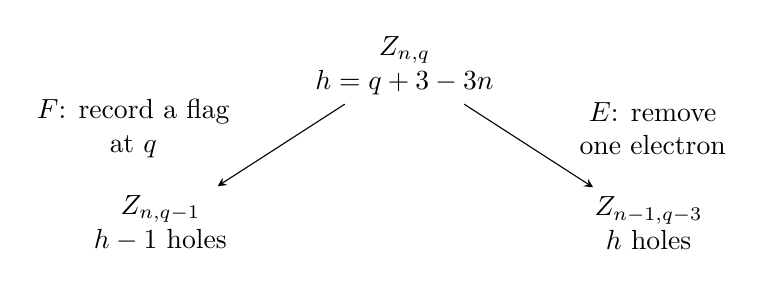
\begin{tikzpicture}[every node/.style={align=center},>=stealth]
 \node (root) at (0,0) {$Z_{n,q}$\\$h=q+3-3n$};
 \node (left) at (-3.1,-2) {$Z_{n,q-1}$\\$h-1$ holes};
 \node (right) at (3.1,-2) {$Z_{n-1,q-3}$\\$h$ holes};
 \draw[->] (root) -- (left);
 \draw[->] (root) -- (right);
 \node[anchor=east] at (-2.1,-0.8) {$F$: record a flag\\at $q$};
 \node[anchor=west] at (2.1,-0.8) {$E$: remove\\one electron};
\end{tikzpicture}
\caption{One step of the orthogonal decomposition.  The displayed spaces
are coordinate spaces for the two branches.  A flag is a record of an
$F$ step; it is not a measured position of a quasihole.}
\label{fig:flags-branches}
\end{figure}

The remaining issue in this decomposition is analytic.  A polar
decomposition need not be local when its nonzero singular values approach
zero.  The next lemma rules out that problem uniformly in the flux.

\subsection{A local polar map}

\begin{lemma}[Occupation gap and local representatives]
\label{lem:flags-polar}
There is $\varepsilon>0$, independent of $q$ and of the number sector,
such that
\begin{equation}
 P_q n_qP_q\geq\varepsilon P_{\mathcal E_q},
 \qquad \mathcal E_q=\bigoplus_n\mathcal E_{n,q}.
 \label{eq:flags-occupation-gap}
\end{equation}
The polar map $\mathsf T_q$ and the projections onto the two branches, restricted
to $Z_q$, have bounded physical representatives rapidly localized at the
south pole.  The representatives preserve $Z_q$ and its orthogonal
complement.  They have respectively the number and index grades of $c_q$
and of the identity.
\end{lemma}

\begin{proof}
We first prove the singular-value bound, keeping track of the restriction
of pair rows.  The normalized rows are
\[
 B_{q,b}=\sum_{\substack{0\leq i<j\leq q\\i+j=b}}
 a_{q,b}(i,j)c_jc_i,\qquad
 a_{q,b}(i,j)=
 \frac{(j-i)\sqrt{\binom qi\binom qj}}
 {\sqrt{q\binom{2q-2}{b-1}}},\quad 1\leq b\leq2q-1.
\]
For completeness, their normalization follows by taking coefficients in
\[
 \sum_{i<j}(j-i)^2\binom qi\binom qj x^{i+j}
 =(1+x)^q(x\partial_x)^2(1+x)^q
  -\bigl((x\partial_x)(1+x)^q\bigr)^2
 =qx(1+x)^{2q-2}.
\]
If a row contains orbital $q$, put $k=2q-b$.  Its removed coefficient
mass is
\[
 p_{q,k}=\frac{k\binom{q-1}{k-1}}{\binom{2q-2}{k-1}}.
\]
Here $p_{q,1}=p_{q,2}=1$, and
\[
 \frac{p_{q,k+1}}{p_{q,k}}
 =\frac{(k+1)(q-k)}{k(2q-k-1)}\leq1.
\]
It follows that every row with a retained pair has retained mass
\begin{equation}
 r_{q,b}=\sum_{\substack{i<j<q\\i+j=b}}|a_{q,b}(i,j)|^2
 \geq\frac{q}{4q-6}\geq\frac14.
 \label{eq:flags-retained-mass}
\end{equation}
Rows with no coefficient at $q$ have mass one.  The two top rows retain
no pair and are omitted.

For $d=1$, the pinning weights obey
$g_j=\tfrac12\log((q-j)/q)$.  Multiplication of its coefficients by
$e^{-g_i-g_j}$, followed by normalization, turns a flux-$(q-1)$ row into
the normalized retained flux-$q$ row.  More precisely, if
$B_{q,b}^{\mathrm{ret}}$ denotes the row with the coefficient at orbital
$q$ deleted, then
$B_{q,b}^{\mathrm{ret}}=\sqrt{r_{q,b}}B_{q,1,b}(1)$, in the notation
of Equation~\eqref{eq:pinning-rows}.  Let $\delta>0$ be the uniform
endpoint gap from Lemma~\ref{pinning:uniform-gap}.  By
\eqref{eq:flags-retained-mass}, the Hamiltonian compressed to the
south-empty sector has a gap at least $\delta/4$ above
$\bigoplus_n\mathcal F_{n,q}$.

The CAR give the exact identity
\[
 \sum_b[B_{q,b},n_q]^*[B_{q,b},n_q]
 =n_q\sum_{k=1}^{q}p_{q,k}n_{q-k}.
\]
The coefficient sum is
\[
 \sum_{k=1}^{q}p_{q,k}=\frac{4q-2}{q+1}<4.
\]
One way to see this is to write
$p_{q,k}=k\binom{2q-k-1}{q-1}/\binom{2q-2}{q-1}$ and apply the
hockey-stick identity twice.  For $\psi\in Z_q$, the two top singleton
rows also imply $c_{q-1}c_q\psi=c_{q-2}c_q\psi=0$.  Hence
\begin{equation}
 \sum_b\|[B_{q,b},n_q]\psi\|^2
 \leq2\|c_q\psi\|^2.
 \label{eq:flags-emptying-energy}
\end{equation}
Let $Q=1-n_q$ and let $P_F$ project onto
$\bigoplus_n\mathcal F_{n,q}$.  Since
$B_{q,b}\psi=0$, the restricted gap gives
\[
 \frac\delta4\|Q\psi-P_F\psi\|^2
 \leq\sum_b\|B_{q,b}Q\psi\|^2
 \leq2\|c_q\psi\|^2.
\]
The occupied and vacant components are orthogonal, so
\[
 \|\psi-P_F\psi\|^2
 \leq(1+8/\delta)\|c_q\psi\|^2.
\]
Thus \eqref{eq:flags-occupation-gap} holds with
$\varepsilon=\delta/(\delta+8)$.

To construct local representatives, take a real smooth frequency cutoff
$\chi$ equal to one near zero and supported strictly inside the uniform
unperturbed gap.  Apply its time filter to $c_q$:
\[
 A_q=\int_{\mathbb R}\widehat\chi(t)
          e^{itH_q}c_qe^{-itH_q}\,dt,
\]
with the Fourier normalization incorporated into $\widehat\chi$.
Contraction preserves zero modes.  The cutoff therefore gives
$A_qP_q=c_qP_q$ and $[A_q,P_q]=0$.  The local calculus makes $A_q$
rapidly localized at the south pole, with uniform constants.  Choose a
smooth function $\eta$ on a fixed interval containing the spectrum of
$A_q^*A_q$, equal to zero near zero and to $x^{-1/2}$ for
$x\geq\varepsilon$.  Then
\[
 \widetilde{\mathsf T}_q=A_q\eta(A_q^*A_q)
\]
is rapidly localized by smooth functional calculus and agrees with
$\mathsf T_q$ on $Z_q$.  Its products
$\widetilde{\mathsf T}_q^*\widetilde{\mathsf T}_q$ and
$1-\widetilde{\mathsf T}_q^*\widetilde{\mathsf T}_q$ represent the branch projections on
$Z_q$.  The construction preserves number and index grades because
$H_q$ preserves both and $A_q^*A_q$ has grade zero.  It also preserves
$P_q$ in both directions.  No claim about a spectral gap of
$A_q^*A_q$ outside $Z_q$ is needed: $\eta$ is smooth on that entire
spectral interval.
\end{proof}

\subsection{One-step comparisons}

Write
\[
 K_{q,d}(f)=\mathcal U_{q,d}^*D_q(f)\mathcal U_{q,d}
              -D_{q-d}(f)
\]
on the corresponding smaller zero space.  Proposition~
\ref{pinning:weighted-transport} supplies localized representatives for
these operators, with the stated size and flux-comparison estimates.

\begin{proposition}[Weighted observable at one branch]
\label{prop:flags-weighted-step}
Fix $p\in(0,2)$, $L\geq2$, and $f(j)=f_{L,p}(j)$.  In the orthogonal
coordinates \eqref{eq:flags-two-branches},
\begin{equation}
 \begin{split}
 (J_{q,F}\oplus J_{q,E})^*D_q(f)(J_{q,F}\oplus J_{q,E})
  ={}&\begin{pmatrix}
   D_{q-1}(f)+K_{q,1}(f)&0\\
   0&D_{q-3}(f)+f(q)+K_{q,3}(f)
  \end{pmatrix}+R_q(f),\\
 &\|R_q(f)\|\leq C_p\frac{f(q)}{(L+q)^2}.
 \end{split}
 \label{eq:flags-weighted-step}
\end{equation}
The notation in the left side means the unitary whose columns are the
two branch isometries.  The bound includes the off-diagonal blocks.
For affine $f$ the remainder is zero and $K_{q,d}(f)=0$.
\end{proposition}

\begin{proof}
The $F$ block is the definition of $K_{q,1}(f)$.  For an affine sequence,
the grades of $\mathsf T_q$ give
\[
 D_q(f)\mathsf T_q=\mathsf T_qD_q(f)-f(q)\mathsf T_q
\]
on the zero spaces, and both branch projections commute with $D_q(f)$.
The endpoint transports commute with the number and index operators.
This proves the affine assertion, including the scalar $f(q)$ in $E$.

For a general $f$, subtract its affine Taylor polynomial at $q$.
The remainder $a(j)=f(j)-f(q)-f'(q)(j-q)$ satisfies
\[
 |a(j)|\leq C_p\frac{f(q)}{(L+q)^2}
                   (1+q-j)^{p+4},\qquad 0\leq j\leq q.
\]
The same polynomial bounds hold for the finite differences needed for
localization.  In the south-pole frame this says that $D_q(a)$ has
one-body interaction size at most $C_pf(q)/(L+q)^2$, times a fixed
polynomial in distance from the pole.  Commuting it with any of the
rapidly localized representatives in Lemma~\ref{lem:flags-polar} thus
has norm at most that size: decompose the representative into ball
shells and sum its arbitrarily high inverse-power tails against this
polynomial.  In the $E$ block use
$\mathsf T_q[D_q(a),\mathsf T_q^*]$; for the off-diagonal blocks use the commutator with
a branch projection.  Compression and the endpoint isometries do not
increase these norms.  This proves \eqref{eq:flags-weighted-step}.
\end{proof}

For a general observable supported far to the north, the polar map
contributes an even smaller error, because its representative is
localized at the opposite pole.  We record the precise form used below.

\begin{lemma}[Northern comparison]
\label{lem:flags-northern-step}
There are fixed $c\geq0$ and $b_0\geq1$ with the following property.
Let $O=O^*$ be neutral, of norm at most one, supported on a slot ball of
radius $r\geq2$ centered at latitude index $m$, and put $u=1+m$.
If $q>C r^{b_0}u$, identify all northern slots in the fluxes being
compared.  The two diagonal branch blocks of $O$ equal
\[
 O+\mathcal D_{q,1}(O)\quad\hbox{and}\quad
 O+\mathcal D_{q,3}(O)
\]
up to a matrix remainder of norm $C_Dq^{-D}$ for every fixed $D$.
Each $\mathcal D_{q,d}(O)$ is neutral and self-adjoint.  If $x$ is its
original center, then, for fixed $c,C_*<\infty$ and every $D>0$,
\begin{equation}
 \begin{split}
 \|\mathcal D_{q,d}(O)\|&\leq Cr^cu/q^2,\\
 \inf_{A_R\in\mathfrak A(B_R(x))}
       \|\mathcal D_{q,d}(O)-A_R\|
  &\leq C_Dr^cu q^{-2}R^{-D}\qquad(R\geq C_*r).
 \end{split}
 \label{eq:flags-northern-size}
\end{equation}
For $|q-q'|\leq2$ and fixed $d$, the difference between these changes,
in common northern slots, obeys the same two estimates with $q^{-2}$
replaced by $q^{-3}$.  The exponent $c$ and core constant $C_*$ are
independent of $D$.
\end{lemma}

\begin{proof}
For $F$, this is Corollary~\ref{pinning:northern-observable}.
Its norm and tail estimates are
Equations~\eqref{eq:pinning-northern-norm} and
\eqref{eq:pinning-northern-tail}; enlarge the fixed core constant to
write the outer ball radius as $R$ instead of $r+R$.
For $E$, commute $O$ through the local representative of $\mathsf T_q$ before
applying that corollary with $d=3$.  The support of $O$ is a distance
comparable with $\sqrt q$ from the south pole when $b_0$ is increased
if necessary.  Rapid locality therefore makes the polar commutator and
the off-branch blocks $O(q^{-D})$ for every $D$.  The same estimate
handles the finitely many trimmed orbitals.  The difference assertion
for the remaining changes is the same-corollary comparison of the
pinning transports at bounded flux difference.
\end{proof}

\subsection{Histories and a linear reference expectation}

Iterate the two branch coordinates until the flux reaches
$q_{\mathrm{stop}}$.  A word $\omega$ records its successive $F$ and
$E$ choices; its terminal number and flux are denoted by $n_\omega$
and $q_\omega$.  The resulting unitary is
\begin{equation}
 \mathcal R_{n,q}:Z_{n,q}\longrightarrow
       \bigoplus_{\omega}Z_{n_\omega,q_\omega}.
 \label{eq:flags-history-map}
\end{equation}
For a fixed readout axis and fixed filters, the maps $J_{q,F}$,
$J_{q,E}$, and $\mathcal R_{n,q}$ are defined on physical Fock spaces
independently of the auxiliary slot frames.  Rebuilding frames outside
the common northern slots changes only the representations used to
prove locality estimates; it does not redefine these maps or their
history coordinates.
An $F$ step taken at flux $b$ records one flag with value $b$.  At a
terminal space we add $q_\omega+3-3n_\omega$ flags, all with value zero.
Let $\mathcal B(\omega)$ be this multiset.  Each word has exactly $h$
flags.  The vacuum follows only $F$ steps, with the same terminal
convention.  We do not resolve the bounded-dimensional terminal space
further.

Fix $a\in(0,2)$.  On the direct sum in
\eqref{eq:flags-history-map}, define the positive diagonal operator
\begin{equation}
 W_m(\omega)=\sum_{b\in\mathcal B(\omega)}
       \min\left\{1,\left(\frac{1+m}{1+b}\right)^a\right\}.
 \label{eq:flags-history-weight}
\end{equation}
Its value is scalar on each terminal summand.  In particular $W_m=0$
on the filled zero space, and $W_m\geq(1+q)^{-a}$ whenever $h>0$.

We next fix the scalar used to center observables.  Put
$q^0=3\lfloor q/3\rfloor$, and let $\Omega_{q^0}$ be the normalized
filled zero mode at that flux.  Embed its one-particle space into $U_q$
by sending orbital $j$ to orbital $j$, and then use the slot embedding
at flux $q$, with the orthogonal complement of the embedded one-particle
space vacant.  Define
\begin{equation}
 \operatorname{ref}_q(O)=
 \langle\Omega_{q^0},O\Omega_{q^0}\rangle
 \label{eq:flags-reference}
\end{equation}
in this padded realization.  This is a positive linear functional of
norm one on the slot algebra.  At $q=q^0$ it is the filled expectation.
For $q^0=0$ the convention is $U_0=\mathbb C$ with its unique normalized
one-electron filled vector.  Outside the common northern region only
linearity, the norm-one bound, and the exact filled expectation at
$q=q^0$ will be used.

\begin{lemma}[Compatibility of reference expectations]
\label{lem:flags-reference-compatibility}
Let two fluxes $q,q'$ use common northern slots, and let
$s\leq\min(q,q')$.  Embed a fixed vector of $\mathcal F_s$ into either
system by the same orbital labels, with the orthogonal complement of
the embedded one-particle space vacant.  The two states have identical
expectations on the algebra of common northern slots.  In particular,
references at fluxes with the same nearest lower filled flux agree on
that algebra.
\end{lemma}

\begin{proof}
Expand a slot observable into normally ordered CAR monomials.  Its
expectation in an embedded state is a linear combination of the state's
normally ordered orbital correlations.  The coefficients use only the
analysis-frame entries of the slots occurring in the monomial.  Entries
at orbital labels above $s$ contribute zero, because those orbitals are
vacant.  At labels at most $s$, the common northern frame entries are
identical.  Thus every monomial has the same expectation in both
realizations.  This also proves the assertion after physical compression
of the slot observable, which leaves these matrix elements unchanged.
\end{proof}

The parent and its $E$ child use filled states at $q^0$ and $q^0-3$,
respectively.  Their expectations are related by the filled $E$ step.
By contrast, the references at $q-3$ and $q^0-3$ use the same filled
state and agree on common northern slots by
Lemma~\ref{lem:flags-reference-compatibility}.  For a rapidly localized
operator, apply this exact identity to a truncation supported in those
slots; the remaining difference is at most twice the truncation error.
The common-frame construction permits these conventions for every
frame entering a comparison, with uniform estimates.

\begin{theorem}[Local observables in history coordinates]
\label{thm:flags-local-readout}
For every fixed $a\in(0,2)$ there are $B,C<\infty$ such that the
following holds uniformly in $n,q$ and in the allowed slot frames.
Let $O=O^*$ be a neutral slot observable of norm at most one, supported
in a ball of radius $r\geq2$ with center of latitude index $m$.  Its
compression to $Z_{n,q}$ satisfies
\begin{equation}
 \pm\left(
 \mathcal R_{n,q}P_{n,q}OP_{n,q}\mathcal R_{n,q}^*
       -\operatorname{ref}_q(O)I\right)
 \leq C r^B W_m.
 \label{eq:flags-local-readout}
\end{equation}
Here $P_{n,q}$ denotes the zero-space projection in the number-$n$
sector.  More generally, for a convergent decomposition
$A=\sum_\nu A_\nu$ into neutral self-adjoint observables supported in
balls about the same center, of respective radii $r_\nu\geq2$, the
right side can be replaced by
$CW_m\sum_\nu r_\nu^B\|A_\nu\|$.
\end{theorem}

\begin{proof}
The proof keeps $O$ unchanged while descending through common northern
slots.  Only the small changes caused by each transport are estimated
inductively.  This distinction prevents an increasing radius from
being assigned repeatedly to the original observable.

We first describe the centered one-step identities under the northern
condition of Lemma~\ref{lem:flags-northern-step}.  For an $E$ step
put $t=q-3$, so $t^0=q^0-3$, and write $R_{q,E}(O)$ for its uncentered
polar remainder in Lemma~\ref{lem:flags-northern-step}.  The filled
$E$ step at $q^0$, together with compatibility of the northern
references, gives the exact scalar identity
\[
 \operatorname{ref}_q(O)-\operatorname{ref}_t(O)
 =\operatorname{ref}_{t^0}\bigl(
     \mathcal D_{q^0,3}(O)+R_{q^0,E}(O)\bigr).
\]
Thus the parent-to-child reference change is determined by a filled
step.  Define
\[
 \begin{split}
 R_{q,E}'(O)&=R_{q,E}(O)
           -\operatorname{ref}_{t^0}(R_{q^0,E}(O))I,\\
 s_q(O)&=\operatorname{ref}_t(\mathcal D_{q,3}(O))
         -\operatorname{ref}_{t^0}(\mathcal D_{q^0,3}(O)).
 \end{split}
\]
The references in the second line use the same filled state.
Lemma~\ref{lem:flags-reference-compatibility}, first on common northern
slots and then on rapid tails by norm approximation, therefore gives
\[
 s_q(O)=\operatorname{ref}_{t^0}\bigl(
     \mathcal D_{q,3}(O)-\mathcal D_{q^0,3}(O)\bigr)
     +O(q^{-D}).
\]
The bounded-flux comparison in Lemma~\ref{lem:flags-northern-step}
supplies the additional factor $q^{-1}$.  Substituting these scalar
identities into the branch comparison yields
\begin{equation}
 \begin{split}
 J_{q,E}^*(O-\operatorname{ref}_q(O))J_{q,E}
 ={}&(O-\operatorname{ref}_t(O))
    +\bigl(\mathcal D_{q,3}(O)
               -\operatorname{ref}_t(\mathcal D_{q,3}(O))\bigr)\\
    &+s_q(O)I+R_{q,E}'(O),\\
 |s_q(O)|\leq{}&Cr^c u/q^3+C_Dq^{-D},\qquad
 \|R_{q,E}'(O)\|\leq C_Dq^{-D}.
 \end{split}
 \label{eq:flags-centered-E}
\end{equation}
Here and below the symbols denote compressions to the relevant child
zero space.  When $h=0$ the comparison is its own filled calibration,
so all centered contributions vanish exactly.

For an $F$ step, $t=q-1$.  The nearest smaller filled fluxes are either
identical or differ by three.  In the latter case apply the filled
$E$ comparison just used.  Together with
\eqref{eq:flags-northern-size}, this proves
\begin{equation}
 J_{q,F}^*(O-\operatorname{ref}_q(O))J_{q,F}
 =O-\operatorname{ref}_t(O)+S_{q,F}(O),\qquad
 \|S_{q,F}(O)\|\leq Cr^cu/q^2+C_Dq^{-D}.
 \label{eq:flags-centered-F}
\end{equation}
The off-diagonal blocks have norm $C_Dq^{-D}$.  An $F$ step already
records a flag, so its entire error will be charged to that flag.

Here is a uniform closure argument, including the parameter choices.
Let $c,b_0$ be as in Lemma~\ref{lem:flags-northern-step}.  Choose
$b>\max\{b_0,c\}$, then choose $B>\max\{ab,c\}$ large enough to
absorb the fixed polynomial costs of the local calculus.  A constant
$M$ will be fixed after $B$.  Set
\[
 \tau=Mr^b u.
\]
If $q\leq\tau$ and $h>0$, every flag has $b'\leq q$, so
\[
 W_m\geq(2Mr^b)^{-a}I.
\]
The norm bound $\|O-\operatorname{ref}_q(O)\|\leq2$ proves
\eqref{eq:flags-local-readout} in this region with constant
$2(2M)^a$.  When $h=0$ the centered compression is zero.  Increasing
$M$ includes all stopping cases in this argument.

Fix a finite $Q$, and let $K_Q$ be the least constant in
\eqref{eq:flags-local-readout} for fluxes at most $Q$, with the
chosen $B$, all number sectors, and all allowed frames.  This number
is finite: for $h>0$ use $W_m\geq(1+Q)^{-a}$, while the filled
compression is exactly centered.  We prove
\begin{equation}
 K_Q\leq C_M+\frac12K_Q
 \label{eq:flags-bootstrap-constant}
\end{equation}
with $C_M$ independent of $Q$.

Suppose $q>\tau$.  Expand the unchanged $O$ down the branching tree,
using \eqref{eq:flags-centered-E} and
\eqref{eq:flags-centered-F}, until the current flux is at most
$\tau$.  The original northern slots, center, and radius are unchanged
through this part of the descent.  The terminal comparisons have just
been bounded.  In an $E$ child, decompose
$\mathcal D_{q,3}(O)$ into its core and dyadic ball shells, all centered
at $m$.  Equation~\eqref{eq:pinning-northern-moment}, with a tail order
larger than $B+2$, gives
\[
 \sum_\nu r_\nu^B\|\mathcal D_{q,3}(O)_\nu\|
 \leq C(B)r^{B+c}u/q^2.
\]
Applying the definition of $K_Q$ to each smaller-flux shell, and using
linearity of the reference, bounds its centered contribution by
\[
 K_QC(B)r^{B+c}u/q^2
\]
times the remaining history weight in that child.  Along any word,
the flux strictly decreases; thus
\[
 \sum_{q'>\tau}\frac{u}{(q')^2}\leq C\frac{u}{\tau}
       =\frac{C}{Mr^b}.
\]
Consequently all induction-dependent contributions are bounded by
\[
 K_Q\frac{C(B)}M r^{B+c-b}W_m.
\]
Choose $M$ so large that this is at most
$\tfrac12 K_Qr^BW_m$.  This choice is possible because $b>c$ and
$r\geq2$.

We verify that the other errors have a bound independent of $K_Q$.
At a node with positive remaining hole number, its identity is bounded
by the sum of the identities assigned to its remaining flags.  A
scalar electron error may therefore be charged to every such flag.
For a flag at $\ell$, the total charge from ancestors in
\eqref{eq:flags-centered-E} is at most
\begin{equation}
 C\frac{r^cu}{\max\{\tau,1+\ell\}^2}.
 \label{eq:flags-scalar-tail}
\end{equation}
The $F$ error in \eqref{eq:flags-centered-F} occurs at its own flag
and obeys the same bound, up to a fixed constant.  Write
$w_\ell=\min\{1,(u/(1+\ell))^a\}$.  Since $a<2$ and $\tau=Mr^bu$,
\[
 \frac{r^cu}{\max\{\tau,1+\ell\}^2}
 \leq C M^{a-2}r^{c+b(a-2)}w_\ell
 \leq C_M r^B w_\ell.
\]
The $q^{-D}$ remainders, including the off-diagonal blocks, obey the
same estimate after choosing $D>a+2$.  For a self-adjoint off-diagonal
block, its norm bounds the full block matrix above and below by that
norm times the identity at its node, so the same charge applies.
Nodes with $h=0$ contribute nothing, by the exact centered filled
identity.  Summation of these diagonal bounds along words proves
\eqref{eq:flags-bootstrap-constant}.

It follows that $K_Q\leq2C_M$ for every $Q$, proving the uniform
claim.  Finally, the assertion for $A=\sum_\nu A_\nu$ follows by
linearity of the reference and by summing the form inequalities.
\end{proof}

The theorem estimates a compression to the zero spaces.  It does not
claim that ordinary local fluctuations vanish in the filled state.
It also applies to coherent superpositions of histories: all charges
above are diagonal operator bounds, rather than bounds conditional on
a classical choice of word.

\subsection{Rotation averaging in a one-hole space}

The history estimate still depends on a chosen readout axis.  In this
subsection, a one-hole space means a space with quasihole degree $h=1$.
Representation theory then removes the axis dependence and yields an
integrated estimate with no factor of the sphere area.

\begin{corollary}[One-hole comparison]
\label{cor:flags-one-hole}
Suppose $h=1$, equivalently $q=3n-2$.  Let $\psi,\phi$ be any two unit
vectors in $Z_{n,q}$.  Let $\{O_x\}$ be a measurable family of neutral
self-adjoint observables of norm at most one, supported in balls of a
fixed radius $r\geq2$ about $x$, with center measure of bounded density.
There are constants $C,B'<\infty$, independent of $n,q$, such that
\begin{equation}
 \int\left|
 \langle\psi,O_x\psi\rangle-\langle\phi,O_x\phi\rangle
 \right|\,dx\leq Cr^{B'}.
 \label{eq:flags-one-hole}
\end{equation}
The same conclusion holds for rapidly localized families, with the
right side bounded by the corresponding fixed rapid-locality seminorm.
For a family whose norms are bounded by $A$, multiply the right side by
$A$.
\end{corollary}

\begin{proof}
Choose $a\in(1,2)$ in Theorem~\ref{thm:flags-local-readout}.  The
symmetric-polynomial factor in \eqref{eq:flags-polynomial-space} has
degree one in each variable.  It is the irreducible spin-$n/2$
representation, so $Z_{n,q}$ is irreducible and has dimension $n+1$.

When $h=1$, an $F$ branch has $h=0$ and hence dimension one.  Before
that branch all steps are $E$, which lower the flux by three.
Therefore at most one one-dimensional history has a flag at any
specified nonterminal flux.  The history that reaches the stopping
region without an $F$ step has bounded terminal dimension.  It follows
that, as an operator on $Z_{n,q}$,
\begin{equation}
 \operatorname{Tr}(W_0)
 \leq C+\sum_{b\geq0}(1+b)^{-a}\leq C_a.
 \label{eq:flags-one-hole-trace}
\end{equation}
The trace is unchanged on conjugating back to the physical zero space.
Write $\widehat W_0=\mathcal R_{n,q}^*W_0\mathcal R_{n,q}$ for that
physical operator.

Let $V_q(g)$ denote the rotation representation, with normalized Haar
measure $dg$.  Schur's lemma gives
\[
 \int_{\mathrm{SU}(2)}V_q(g)\widehat W_0V_q(g)^*\,dg
 =\frac{\operatorname{Tr}(\widehat W_0)}{n+1}I.
\]
For each rotation use the readout axis whose north pole is the image
of the original north pole.  Precisely, write
$x(g)=g\cdot\mathrm{north}$ and
$W^{g}=V_q(g)\widehat W_0V_q(g)^*$.
Use the rotated frame and rotated branch construction at $x(g)$.
Theorem~\ref{thm:flags-local-readout}, applied to $O_{x(g)}$, gives
\[
 \bigl|\langle\psi,O_{x(g)}\psi\rangle
       -\langle\phi,O_{x(g)}\phi\rangle\bigr|
 \leq Cr^{B'}\bigl(\langle\psi,W^g\psi\rangle
                    +\langle\phi,W^g\phi\rangle\bigr).
\]
The two reference expectations cancel in this inequality.
Changes between local frames cost only a fixed polynomial in $r$ by
the local calculus.  Integrating rotations and multiplying by the
sphere area yields at most
$Cr^{B'}q\operatorname{Tr}(W_0)/(n+1)$, which is uniformly bounded
because $q=3n-2$.  For any center measure with bounded mass in unit
balls, spread the mass at each center over a ball of fixed radius.
The resulting density relative to area is bounded uniformly.  The
operator originally assigned to $x$ is supported in a ball of radius
$r+1$ about every point in that spreading ball, so the same pointwise
bound applies before integration.  This reduces the general center
measure to the area estimate.  Finally, summing ball shells proves the
assertion for rapid families.
\end{proof}
